\documentclass[10pt, a4paper, twoside]{article}

% Set up the standard margins for the document
% 42.2 left & 15.5 right is same as Forsling, Neymark
% 21.3 top  & 20 bottom is same as Olofsson
\usepackage[left=19.5mm, right=19.5mm, top=21.3mm, bottom=20mm]{geometry}

% Input file character encoding (kinda useless if we don't
% use åäö and stuff, but it doesn't hurt to have it)
\usepackage[utf8]{inputenc}
%\usepackage[swedish]{babel}

% Block Comments
\usepackage{comment}

\usepackage{float}

% No indentation in new paragraph
\usepackage{parskip}

% To include graphics
\usepackage{graphicx}

% More mathematical symbols and fonts
\usepackage{amsmath}
\usepackage{amsfonts}
\usepackage{amssymb}

% Simple list
\usepackage[ampersand]{easylist}
\ListProperties(Hide=100, Hang=true, Progressive=5ex, Style*=$\bullet$ ,
Style2*=-- ,Style3*=$\circ$ ,Style4*=\tiny$\blacksquare$ )


% Clickable internal links
\usepackage{hyperref}
\usepackage[all]{hypcap} % without this the link takes you to the caption, not the top of the image
\hypersetup{ % Settings for links in documnet
	setpagesize = false, % Don't allow hyperref to change page size. Tips från Micke Olofsson
	colorlinks = true,   % No boxes around links
	linkcolor = black,citecolor = black,filecolor = black,urlcolor = black, % don't color links
}

% To include to first page pdf file
\usepackage{pdfpages}

% Add section number to equation and figure number (ex: 5.11 instead of simply 11)
\numberwithin{equation}{subsection}
\numberwithin{figure}{section}
\numberwithin{table}{section}

% Show program code listings in document
\usepackage{listings}

%
% Header stuff
%
\usepackage{fancyhdr}
\setlength{\headheight}{15pt}

\fancyhf{}
\fancyhead[LE, RO]{\thepage}
\fancyhead[RE]{TSBB15 2013: User Manual}
\fancyhead[LO]{Kitchen Occupation}

\fancypagestyle{plain}{ %
\fancyhf{} % remove everything
\renewcommand{\headrulewidth}{0pt} % remove lines as well
\renewcommand{\footrulewidth}{0pt}}
%
% End header stuff
%




\begin{document}

% First page

\includepdf{Cover/cover.pdf}


% Project identity page
\newpage
\pagestyle{fancy}
\pagenumbering{roman}
\setcounter{page}{2} % sets the current page number to 2 

\begin{center}
    \vspace*{4\baselineskip}

	\textbf{\huge Project Kitchen Occupation} \\
	\vspace*{0.5\baselineskip}
	Bilder och Grafik CDIO, HT 2013 \\
	Department of Electrical Engineering (ISY), Link\"{o}ping University
	
	\vspace*{2\baselineskip}
	\textbf{\LARGE Participants}


	{\footnotesize 
	\begin{tabular}{|p{2.7cm}|p{1cm}|p{5cm}|p{2cm}|p{3.4cm}|}
		\hline
		\textbf{Name} & \textbf{Tag} & \textbf{Responsibilities} & \textbf{Phone} & \textbf{E-mail} \\
		\hline
		Mattias Tiger & MT & Project manager & 073--695\,71\,53 & matti166@student.liu.se \\
		\hline
		Erik Fall & EF & -- & 076--186\,98\,84 & erifa226@student.liu.se \\
		\hline
		Gustav Häger & GH & System integration & 070--649\,03\,97 & gusha124@student.liu.se \\
		\hline
		Malin Rudin & MR & -- & 073--800\,35\,77 & malru103@student.liu.se \\
		\hline
		Alexander Sjöholm & AS & -- & 076--225\,11\,74 & alesj050@student.liu.se \\
		\hline
		Martin Svensson & MS & Documentation & 070--289\,01\,49 & marsv106@student.liu.se \\
		\hline
		Nikolaus West & NW & Testing & 073--698\,92\,60 & nikwe491@student.liu.se \\
		\hline
	\end{tabular}
	}

{\footnotesize 
\vspace{0.5\baselineskip}
\textbf{Homepage}: TBA \\
\vspace{1\baselineskip}

\textbf{Customer}: Joakim Nejdeby, Link\"{o}ping University, Origo 3154 \\
\textbf{Customer contact}: 013--28\,17\,57, joakim.nejdeby@liu.se \\
\textbf{Project supervisor}: Fahad Khan, Link\"{o}ping University, fahad.khan@liu.se \\
\textbf{Examiner}: Michael Felsberg, michael.felsberg@liu.se \\
}

\end{center}



% table of contents
\newpage
\tableofcontents
\listoffigures
\listoftables

% list of figures
%\newpage
%\listoffigures


% Document history page
\newpage
\vspace*{5\baselineskip}

\begin{center}
\textbf{\LARGE Document history}

{ \footnotesize 
\begin{tabular}{|p{1cm}|p{2.0cm}|p{5cm}|p{1.5cm}|p{2cm}|}
	\hline

	\textbf{Version} & \textbf{Date} & \textbf{Changes} & \textbf{Sign} & \textbf{Reviewed} \\
	
	\hline
	0.1 & 2013--12--13 & Initial draft & MS & MT\\
	
	\hline
	 &  &  &  &  \\
	
	\hline
\end{tabular}
}
\end{center}


% Blank page
%\newpage
%\thispagestyle{empty}
%\mbox{}



%
% Content start
%
\newpage
\pagenumbering{arabic}

\newpage
\section{Installing the system}
\label{sec:installation}
\subsection{Hardware}
Each Kinect camera must be installed above a door with no overlapping view shared with any other Kinect camera. The Kinect must point down or slightly angled towards the room. A minimum distance of 50 cm is required from the lense of the Kinect and the top of the door. Each Kinect must be connected to a power source, and to a device running the system software using USB.

\subsection{Software}
There are two versions of the software, one with a calibration and configuration GUI and one lightweight version without a GUI. In order for the lightweight version to work a configuration file, persumably generated by the GUI version, is required. The configuration file is best generated using the configuration program, and then copied to the system running the non-GUI variant. \\

Linux, OS-X or Windows is required on the machine running the software. At least one Kinect camera must be connected before starting the software. More than one Kinect camear is currently only working on Linux and OS-X. Some software libraires are required to compile the program, these are listed in table \ref{reqSoftware}. \\

\begin{table} [hbt]
\begin{center}
  \begin{tabular}{ | l | l | }
    \hline
    \textbf{Software} & \textbf{Comments} \\ \hline
    OpenCV2 & Needed for general image processing  \\ \hline
    libFreenect & Needed for communication with kinect on unix like systems  \\ \hline
    OpenNI & Needed for communication with kinect on windows systems  \\ \hline
    libCurl & Needed to send http requests to the report API \\ \hline
    QT5 & Needed for the gui code, not used in headless variant \\ \hline
  \end{tabular}
  \label{reqSoftware}
  \caption{Software libraries requried.}
\end{center}
\end{table}
\newpage

\section{Setting up the system}
The easiest way to setup the system is by using the GUI. Here the main settings can be adjusted. However, there are some advanced settings that can only be adjusted in the configuration file. More on this later. 

\subsection{Calibration}
\label{sec:setup}
The system can be calibrated using the GUI for the most common calibration task. Using the config file all parameters are accessable for further calibration.

\subsection{GUI}
A threshold level is used to adjust the system for the current installation height of the camera. It sets a configuration parameter called lowestDistanceOverFloor. This is the limit of how short a person can be. The threshold should be set so that a "normal" person’s chest is not removed by the thresholding.

\begin{figure}[htb]
	\centering
	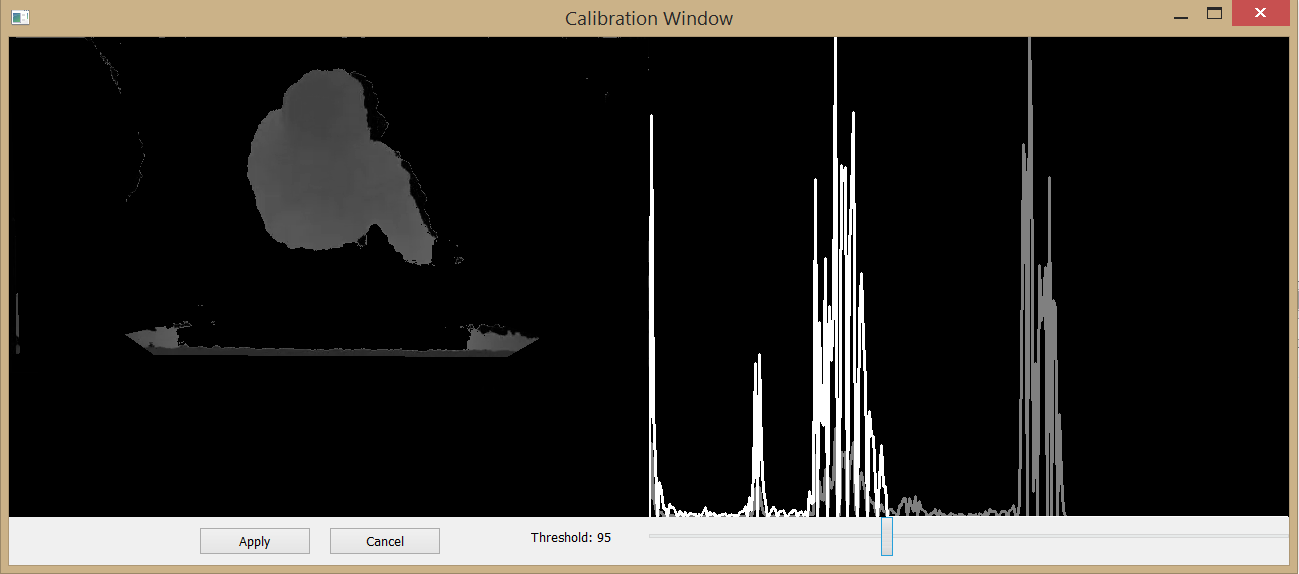
\includegraphics[width=\linewidth]{images/Calibration.png}
	\caption[Overview of the entire system]{\textit{Calibrating the lowestDistanceOverFloor threshold. A histogram i shown to help the user to se how much off different heights are present in the image. The selected heights are gray shaded.}}
	\label{fig:lowestDistanceOverFloor_calibration}  %Skapar referens till figuren
\end{figure}

\newpage
\subsection{Config file}
The config file used by the algorithm pipeline is called \textit{dense\_conf.yml}. In it any configurable variable in any algorithm currently selected to be in the pipeline can be specified. The pipeline itself can also be specified, allowing fo rapid swapping of algorithms. The most useful variables in the current pipeline are shown in table \ref{table:commonVariables}.\\

\begin{table}[hbt]
	\begin{tabular}{ | l | l | p{7.5cm} | }
	    \hline
	    \textbf{Variable} & \textbf{Algorithm/Program-part} & \textbf{Description} \\ \hline
	    runFromFile & Network & If set to 1, the video sources are files found in the paths \textit{videoFilePaths}.  \\ \hline
	    videoFilePaths & Network & The paths to the video files used if running from file.  \\ \hline
	    useKinect & Network & If set to 1, the video sources are from Microsof Kinect cameras. \\ \hline
	    TrackingMaximumDistance & Tracking & The maximum distance an object can be considered to have moved since last frame. \\ \hline
	    TrackingMinimzumLifeSpan & Tracking & The minimal time (in \# frames) a potential object must have existed (and been tracked) before it is considered a real object. \\ \hline
	    TrackingMaximumTimeLost & Tracking & The maximum time (in \# frames) an object is allowed to be lost before it is forgotten. \\ \hline
	    lowestDistanceOverFloor & Kinect Segmentation & The limit (height units) of how short a person can be. Set this variable using the GUI calibration utility described previously. \\ \hline
	    webServerUrl & Network & The address to the web service to which results are reported. \\ \hline
	\end{tabular}
	\label{table:commonVariables}
	\caption{The most useful and common variables in the current pipeline.}
\end{table}

\newpage
Currently the pipeline consists of two major algorithms: \textit{ImageProcessor} and \textit{Analytics}. These in turn have several sub-algorithms that are executed in the order specified in the config file. The current pipeline is structured in the following way: \\
\hspace*{0.5cm}\textit{ImageProcessor:\\
\hspace*{1cm}- KinectSegmentation\\
\hspace*{1cm}- TrackingBruteForce}\\
\hspace*{0.5cm}\textit{Analytics:\\
\hspace*{1cm}- EntryExitCounter\\
\hspace*{1cm}- FlowEstimator\\
\hspace*{1cm}- QueDetector\\
\hspace*{1cm}- QueSeverityEstimator}\\\\
Any algorithm registed in the system can be used as a subalgorithm for any other algorithm, writing in the config file in the same way as with \textit{KinectSegmentation} being a sub algorithm to \textit{ImageProcessor}. To get an empty algorithm placeholder any none-registerd algorithm name (or variable name) may be used, such as:\\
\hspace*{0.5cm}\textit{UnregisterdName:\\
\hspace*{1cm}- KinectSegmentation\\
\hspace*{1cm}- ...}\\
It can now be used as a sub-algorithm to another algorithm (or placeholder algorithm):\\
\hspace*{0.5cm}\textit{ImageProcessors:\\
\hspace*{1cm}- UnregisterdName\\
\hspace*{1cm}- ...}\\
A placeholder algorithm works by just passing through initialization and processing calls to its sub-algorithms.\\\\
\textbf{Warning: If you do not know what your are doing, do not modify the algorithm pipeline. Some algorithms have requirements which must be provided by earlier algorithms, the system will not run if these are not met. See the code documentation for further details on requirements and effetcs of different algorithms.}


\newpage
\subsection{Configuration}
\label{sec:configuration}
The system can be configured using the GUI. Available configuration settings is checkpoint circles, door mask area, exclusion mask and grayscale height threshold settings. 

The circles should be placed so persons walking into the room inevitable will pass all three lines. They should also be more inside the room compared to the door mask area. A good placement is illustrated in figure \ref{fig:circlePlacement}. Note that the red, most inner circle, includes the upper corners of the door frame. Too small inner circle will cause people to miss it and therefore not detected. 

\begin{figure}[H]
	\centering
	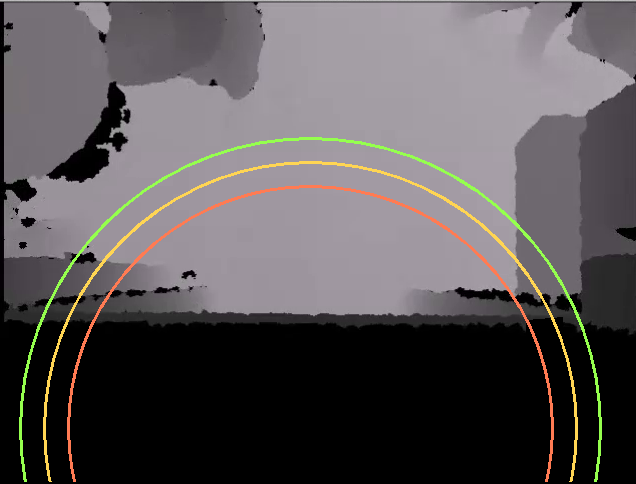
\includegraphics[width=\linewidth]{images/Manual2.png}
	\caption[Circle placment]{\textit{A prefered placement of the circles. }}
	\label{fig:circlePlacement}  %Skapar referens till figuren
\end{figure}

\newpage
The door mask should cover the area close to the door where people appear. It is important to make this area big enough, rather too big than too small. It can, but should not cover the upper, most distant, part of the red circle, figure \ref{fig:doorMask} illustrates this.

\begin{figure}[H]
	\centering
	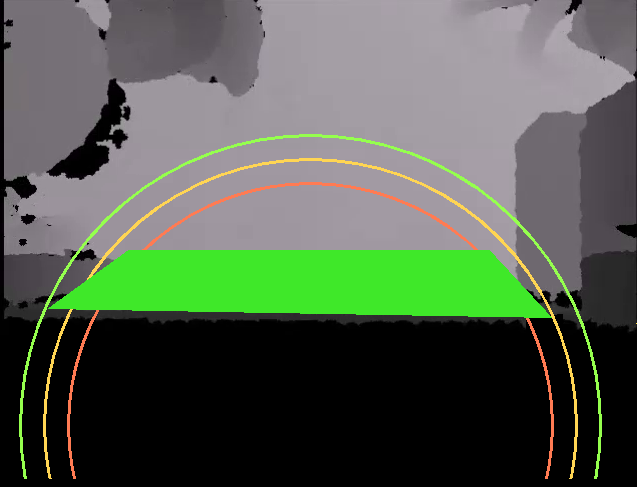
\includegraphics[width=\linewidth]{images/Manual3.png}
	\caption[Exclusion mask]{\textit{The prefered placement of the door mask, the door mask is the green area.}}
	\label{fig:doorMask}  %Skapar referens till figuren
\end{figure}

\newpage
Exclusion masks should cover areas where people can not walk or appear. This could be areas like tables or areas behind the door (walls in this case), figure \ref{fig:exMask} illustrates this. Note that for long usage of the system, movable furniture should not be excluded.

\begin{figure}[H]
	\centering
	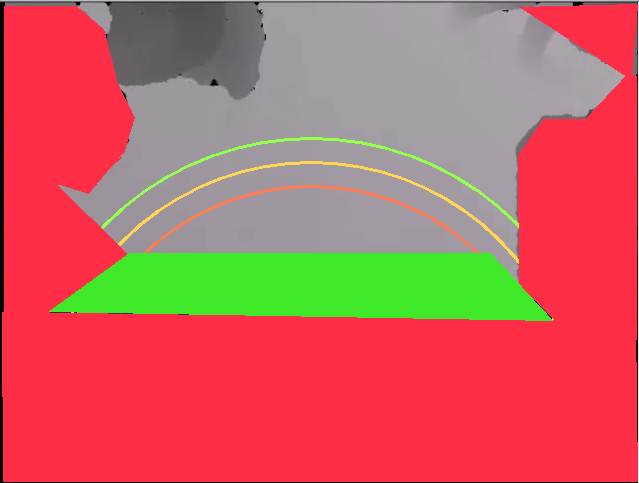
\includegraphics[width=\linewidth]{images/Manual1.png}
	\caption[Exclusion mask]{\textit{Exclusion mask is marked as red. It covers areas where people can not walk or appear.}}
	\label{fig:exMask}  %Skapar referens till figuren
\end{figure}
\newpage


% Force a blank page so the bibliography starts on a new page.
% Comment out if not necessary
%\newpage
%\thispagestyle{fancy}
%\mbox{}
%\begin{thebibliography}{9}
\addcontentsline{toc}{section}{References} % Add an entry for this in the table of contents

\bibitem{Gardel}
	Gardel, A., Bravo, I., Jimenez, P., Lazaro, J.L. \& Torquemada, A.\\
	``\textit{Statistical Background Models with Shadow Detection for Video Based Tracking},''\\ Intelligent Signal Processing, 2007. WISP 2007. IEEE International Symposium on?? Page: 1-6.
	
\bibitem{Zivkovic}
	Zivkovic, Z. \& Heijden, F.\\
	``\textit{Efficient Adaptive Density Estimation per Image Pixel for the Task of Background Subtraction},''\\
	Pattern recognition letters, Vol. 27, No. 7. (2006), pp. 773-780.

\vspace{2cm}
\LARGE{\textbf{EXAMPLE REFERENCES ONLY, REMOVE BEFORE HANDING IN}}
\normalsize
\bibitem{CVBook}
	Sonka, M., Hlavac, V. \& Boyle, R. 
	\emph{Image Processing, Analysis, and Machine Vision}.\\
	Toronto: Thompson Learning,
	cop. 2008, 3rd ed.,
	ISBN 0495244384.
	
\bibitem{Wood}
	Wood, J. (2007)
	``\textit{Statistical Background Models with Shadow Detection for Video Based Tracking},''\\
	Master thesis, Linköping University, Department of Electrical Engineering.	

\bibitem{DSPBook}
	Gustafsson, F., Ljung, L. \& Millnert, M.
	\emph{Signal Processing}.\\
	Studentlitteratur, Lund, Sweden,
	2011, 1st ed.,
	ISBN 978--91--44--05835--1.

\bibitem{MOTA}
	Bernardin, K. \& Stiefelhagen, R (2008)\\
	``\textit{Evaluating Multiple Object Tracking Performance: The CLEAR MOT Metrics},''\\
	Interactive Systems Lab, Institut für Theoretische Informatik,\\
	Universität Karlsruhe, 76131 Karlsruhe, Germany

\bibitem{CAVIAR}
	``\textit{CAVIAR: Context Aware Vision using Image-based Active Recognition},''\\
	EC Funded CAVIAR project/IST 2001 37540\\
	http://homepages.inf.ed.ac.uk/rbf/CAVIAR/
	

%\bibitem{somePaper}
%	Q. Lastname,
%	``Some article title,''
%	\emph{Some scientific journal},
%	vol.~1337, no.~1337,
%	pp.~666--1337,
%	month.~1337.

\end{thebibliography}



\end{document}
